\section{Aufbau}
Der experimentelle Aufbau zur Untersuchung des Photoeffektes ist in Abbildung \ref{fig:aufbau1} dargestellt.
Hier wird zunächst das Licht einer Spektrallampe durch verschiedene optische Geräte und letztendlich durch ein ein Prisma in Spektrallinien aufgebrochen.

\begin{figure}[h]
    \centering
    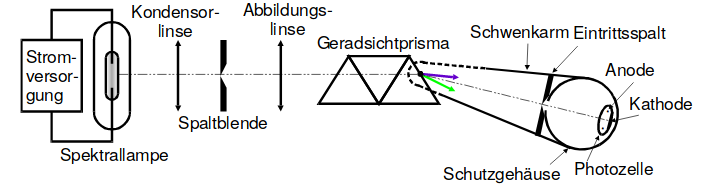
\includegraphics[height=4cm]{Aufbau/Aufbau1.png}
    \caption{.Optischer Aufbau des Experimentes}
    \label{fig:aufbau1}
\end{figure}

Dieses nahezu monochromatische Licht wird dann auf die Photozelle geworfen.
Die Photozelle ist ein vakuumierter Glaskolben, der einerseits die Photokathode enthält, die aus einer auf der Innenseite aufgedampften Metall oder Legierungsschicht besteht.
Andererseits ist kreisförmig um die Photokathode die Auffanganode als Draht angebracht.
In Abbildung \ref{fig:aufbau2} werden diese beiden Elektroden deutlich.
Des Weiteren kann eine Spannung an den beiden Anschlüssen angelegt werden, die die Elektronen entweder beschleunigt oder abbremst.

\begin{figure}[h]
    \centering
    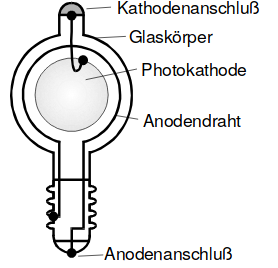
\includegraphics[height=5cm]{Aufbau/Aufbau2.png}
    \caption{.Aufbau der Photozelle}
    \label{fig:aufbau2}
\end{figure}
